\documentclass[../../report.tex]{subfiles}
\begin{document}
\section{Model Architecture}

Understanding and implementing the LSNN was one of the major challenges in this
project. It was very helpful to analyse the experimental code published by
researchers at TU Graz \cite{Bellec2018LSNN, Bellec2020}. Still, large parts of
their implementation had to be rewritten in order to make the LSNN interoperable
with Magenta, and to improve code readability.

\subsection{LSNN cell}

TensorFlow comes bundled with many standard neural network components, e.g.
LSTM. Of course, esoteric modules such as the LSNN must be implemented manually.
In TensorFlow, custom recurrent networks are defined by extending the abstract
\texttt{RNNCell} class, and our LSNN is no exception.

\subsubsection{Constructor arguments}
The LSNN cell has many hyperparameters. Their optimal values depend on the task,
so they have been made configurable via constructor arguments (table
\ref{tab:lsnn-args}).

\begin{table}
  \begin{tabularx}{\textwidth}{ >{\ttfamily}l X }
    num\string_neurons & Number of neurons modelled by this cell \\
    dt & Physical time step per iteration \\
    frac\string_alif & Fraction of neurons with adaptive firing thresholds \\
    num\string_refractory\string_dt & Number of refractory time steps \\
    spike\string_threshold & Threshold membrane potential \\
    potential\string_decay & Membrane potential time constant\footnotemark{} \\
    adaptation\string_decay & Adaptive threshold time
    constant\footnotemark[\value{footnote}] \\
    adaptation\string_magnitude & Adaptive threshold scaling factor \\
    dampening\string_factor & Pseudo-derivative scaling factor \\
  \end{tabularx}
  \caption{LSNN cell constructor arguments.}
  \label{tab:lsnn-args}
\end{table}

\footnotetext{This is a physics concept beyond the scope of this report. In a
nutshell, for a time constant \(\tau\) and a time step \(\delta t\), the decay
factor is given by \(\exp(-\delta t / \tau)\).}

\subsubsection{State}
The state of an LSNN cell is described by a 6-tuple, as detailed in table
\ref{tab:lsnn-state}.

\begin{table}
  \begin{tabularx}{\textwidth}{ >{\ttfamily}l X }
    potentials & Membrane potentials of each neuron \\
    adaptations & Neuronal adaptation level of each neuron \\
    spikes & Spikes emitted in the previous step \\
    refractoriness & Neurons' refractory period counters \\
    num\string_spikes & Running total of spikes for each neuron \\
    num\string_steps & Running total of steps taken by this cell (scalar) \\
  \end{tabularx}
  \caption{LSNN state tuple contents.}
  \label{tab:lsnn-state}
\end{table}

\subsubsection{Input \& output}

The LSNN cell expects to receive binary input spike vectors of arbitrary but
constant size. The output is a binary vector of spikes from internal LSNN
neurons.

\subsubsection{Operation}

Subclasses of \texttt{RNNCell} must implement the \texttt{call} method. It
should take the input and state as arguments, and it should return the output
and next state. The LSNN cell achieves this as follows:

\begin{enumerate}

  \item Input spikes and internal spikes are multiplied with corresponding
  synaptic weight matrices; the results are added to membrane potentials of
  internal neurons.

  \item Membrane potentials and adaptive thresholds are used to determine which
  neurons will spike at this time step.

  \item Spikes are blocked for neurons currently in the refractory period.

  \item Decay factor is applied to membrane potentials.

  \item Decay factor is applied to adaptive thresholds.

  \item Nonzero refractory counters are decremented.

  \item Membrane potentials are reset for neurons spiking in this step.

  \item Adaptive thresholds are increased for ALIF neurons spiking in this step.

  \item Refractory counters are initialised for neurons spiking in this step.

  \item New state vectors are packed into a tuple and returned along with output
  spikes.

\end{enumerate}

\subsection{Utility cells}

In addition to the main LSNN cell, several other components were necessary to
ensure compatibility with Magenta.

\subsubsection{Smoothing the outputs}
With the functionality described so far, it is only possible to extract
spike-based outputs from the LSNN. This is potentially problematic -- some steps
may produce no spikes at all, abstracting away a lot of useful information. To
convert spikes to real valued outputs, it is common to use leaky readout neurons
\cite{Bellec2018LSNN, Bellec2020}. In order to make the code modular, this
functionality was implemented in \texttt{SpikeSmoothingCell}, yet another
subclass of \texttt{RNNCell}. Its \texttt{call} operation can be described by
the following equations:

\begin{align*}
  \mathrm{call}(\bm{x}_t, \bm{s}_t) &= (\bm{y}_t, \bm{s}_{t+1}) \\
  \bm{y}_t &= \bm{x}_t + \lambda\bm{s}_{t} \\
  \bm{s}_{t+1} &= \bm{y}_t
\end{align*}

In other words, this cell uses its state \(\bm{s}\) as a decaying memory of
spike inputs \(\bm{x}\), where the decay factor is \(\lambda \in [0, 1]\). In
each step, this memory is updated with the new spikes and returned as the output
\(\bm{y}\).

\subsubsection{Spiking the inputs}
As it stands, our recurrent network receives melody event inputs in the form of
one-hot encoded vectors. These vectors could be interpreted as spikes directly,
but since SNNs aim to model biological networks, several aspects of realism are
often introduced:

\begin{itemize}
  \item \textbf{Granular time steps}. Each input is presented over several time
  steps, giving the network more time to settle into a new state and letting the
  spikes propagate.

  \item \textbf{Neuron populations}. Instead of feeding the inputs via
  individual neurons, whole populations can be assigned to each distinct input
  category.

  \item \textbf{Randomness}. Spreading a single input over \(t\) time steps and
  populations of \(n\) neurons results in \(tn\) total spikes. To avoid
  oversaturating the network with activity, it is common to make the input
  spikes stochastic by sampling from a Poisson distribution.
\end{itemize}

The above functionality is implemented in \texttt{PoissonSpikeWrapper}, which
again inherits from \texttt{RNNCell}. This class wraps another cell passed via
the constructor, and then intercepts all calls to that cell, dynamically
expanding the inputs as required.

This approach may seem a little odd -- why not encode the melodies into this
expanded form ahead of runtime? That would likely lead to better performance,
but the issue is that the codebase of Magenta is built on the assumption that a
single call to an RNN produces a single output. The modifications proposed above
break this contract, so it would have been necessary to adapt several other
parts of the Magenta library.

\subsection{Putting it all together}

As shown in figure \ref{fig:architecture}, the components described in the
sections above can be used to build a module whose interface is identical to
that of an LSTM. This enables a seamless transition to the LSNN-based variant of
Basic RNN.

It is worth noting that the output of the LSNN is fed into a fully connected
layer. This approach is common in previous work \cite{Bellec2018LSNN,
Bellec2020}. Some may argue that this is a departure from biological realism,
but it is arguably just a convenient method of mapping the internal spikes to an
output vector of desired size. Most importantly, the activation function in this
final layer is linear, meaning that the task of learning non-linearities in
input data is delegated solely to the LSNN.

\begin{figure}
  \centering
  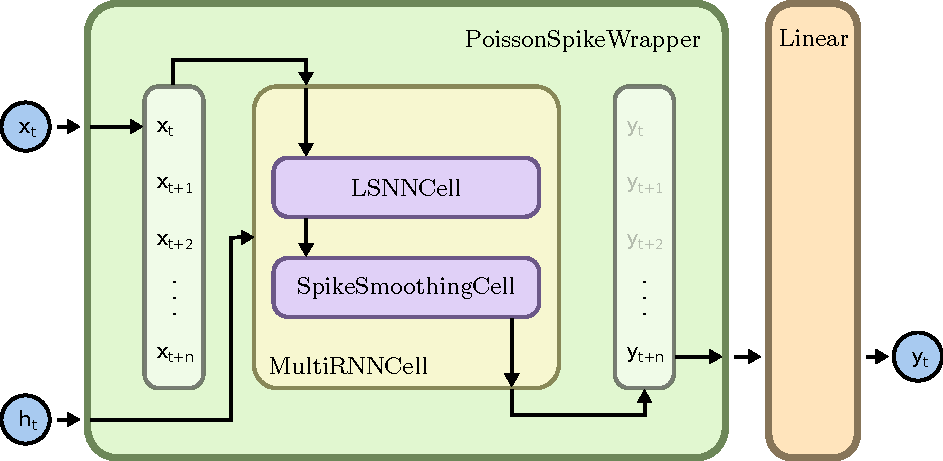
\includegraphics[width=\textwidth]{architecture}
  \caption{Structure of the complete model. Using TensorFlow's RNN utilities,
  one or more LSNN cells can be chained together, ultimately feeding into a
  spike smoothing cell. The composite cell is then wrapped using the custom
  input expander, which transforms a single input \(x_t\) into \(n\) sub-inputs.
  Only the output from the final sub-step \(y_{t+n}\) is surfaced. Lastly, a
  linear layer is used to produce activation values for each output class.}
  \label{fig:architecture}
\end{figure}

\end{document}
